\documentclass[reportComp]{thesis}
\usepackage[cpp,pseudo]{mypackage}

\title{并行分布式计算实验报告}
\subtitle{项目二:最短路径}
\school{数据科学与计算机学院}
\author{陈鸿峥}
\classname{17大数据与人工智能}
\stunum{17341015}
\headercontext{并行分布式计算实验报告}

\begin{document}

\maketitle

\section{题目描述}
现实世界的很多场景中,需要计算最短路径,如导航中的路径规划等,但是如何在大规模路径中快速找出最短路径,是一个具有挑战性的问题。
本项目要求利用MPI + OpenMP,从一个至少包含1万个节点,10万条边的图中,寻找最短路径,边上的权重可随机产生。
统一测试程序的执行时间,进行排名,根据排名计算成绩。

输入数据格式:
\begin{itemize}
	\item 20001个点,7000w+条边,求点0到点20000的最短路径(有解)
	\item 每行3个数,分别为源节点、汇节点、权重(非负)
\end{itemize}

输出:整个路径及路径长度

测试环境:3个节点(同主机的虚机),每个节点两个核心(双核四线程),4G内存,机械硬盘

参照:
\begin{itemize}
\item \url{https://github.com/Lehmannhen/MPI-Dijkstra}
\item \url{https://github.com/laplaceyc/Parallel-Programing}
\end{itemize}

\section{解决方案}
Dijkstra算法是串行求解单源最短路径的常见算法,伪代码如下
\begin{algorithm}[H]
\caption{Sequential Dijkstra SSSP}
\label{alg:dijkstra}
\begin{algorithmic}[1]
\Procedure{Dijkstra}{Graph,Source}
\State Create vertex set $\sQ$\Comment{Initialization}
\For{\textbf{each} vertex in Graph}
\State dist[$v$] $\gets$ INFINITY
\State prev[$v$] $\gets$ UNDEFINED
\State add $v$ to $\sQ$
\EndFor
\State dist[$source$] $\gets$ $0$
\While{$\sQ$ is not empty}\Comment{Dijkstra}
\State $u$ $\gets$ vertex in $\sQ$ with min dist[$u$]
\State remove $u$ from $\sQ$
\For{\textbf{each} neighbor $v$ of $u$}
\State alt $\gets$ dist[$u$] + length($u$,$v$)
\If{alt $<$ dist[$v$]}\Comment{Relaxation}
\State dist[$v$] $\gets$ alt
\State prev[$v$] $\gets$ $u$
\EndIf
\EndFor
\EndWhile
\State\Return{dist[],prev[]}
\EndProcedure
\end{algorithmic}
\end{algorithm}

在本次实验中我采用了两种并行模型,一种是只使用OpenMP,另一种是OpenMP和MPI的结合。
头文件都在\verb'include'文件夹中,并行操作都已封装在\verb'parallel.h'头文件中(如OpenMP的\verb'parallel_for'等),主函数位于\verb'sssp.cpp'中。

\subsection{OpenMP}
\label{sub:openmp}
单机共享内存的并行方式比较简单。
对于两个\verb'for each'部分,就可以使用并行方法进行加速,因为在循环间都没有依赖关系。
还有一个可并行的地方则是在求解距离最小值的部分(伪代码第9行)。

由于我现在的研究方向就是图计算,故本次作业直接复用了我今年以第一作者投稿于SC'19的部分代码(之前已上传过相关的介绍PPT),该代码是开源的\footnote{Krill: An Efficient Concurrent Graph Processing System, \url{https://github.com/chhzh123/Krill}}。

简单来说,优化技术有以下几点。
\begin{itemize}
	\item 将输入文件以字符串形式完全读入内存后,同一并行进行处理,包括并行的初始化、并行的\textbf{基数排序}、并行的赋值等。
	\item 图结构(graph structure\footnote{顶点间的即邻接关系})用\textbf{压缩稀疏行(Compressed Sparse Row, CSR)格式}存储,见图\ref{fig:csr}
	\begin{figure}[H]
	\centering
	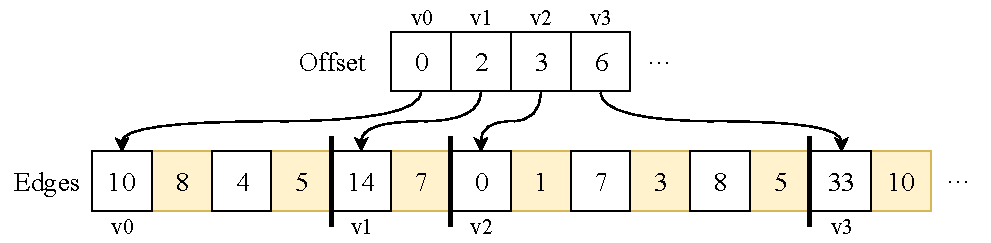
\includegraphics[width=0.8\linewidth]{fig/CSR.pdf}
	\caption{CSR格式}
	\label{fig:csr}
	\end{figure}
	其中,第一个数组存储的是边表的偏移量\verb'offset',第二个数组存储的是每个源结点的邻居(第一项)及边权(第二项)。
	以CSR格式存储,可以使程序具有良好的空间局部性。
	当确定了源结点(当前迭代最小距离点)后,内层循环都是遍历源结点的邻居。
	而在CSR格式中,邻居都是紧密存储的(包括边权),故这可以确保所需的数据都在Cache中,进而大大缩短访存时间。
	当然了,以压缩形式存储,在分布式环境下,通信开销也会小很多。
	\item 图性质(graph property)用一个结构体\verb'DistPack'打包,包含顶点标号\verb'i'、距离向量\verb'dist'、前驱\verb'prev'、访问标记\verb'flag',这样存储同样使得同一个结点的图性质具有良好的局部性。
	\item 注意到最小值函数具有交换律和结合律,故可以利用\textbf{前缀和}(prefix sum\footnote{\url{https://en.wikipedia.org/wiki/Prefix_sum}})进行并行优化,这在代码中体现为\verb'sequence::reduce'。
	通过传入数组\verb'res'、元素个数\verb'n'及作用函数\verb'minPackF',即可进行分组归并计算。
	\item 由于本题只要求求0到20000的最短路径,故当最小路径值为20000对应的结点时,即可进行\textbf{剪枝},提前退出循环。其正确性是由最短路径的最优子结构保证的。
\end{itemize}

可以算得在$p$个核的环境下,并行Dijkstra算法的时间复杂度为$O(n^2/p+\log p)$。

注意,由于测试数据集较小,故这些优化技术很可能不起作用。

\subsection{OpenMP$+$MPI}
第二种方式则是结合共享内存的编程模型OpenMP和消息传递型的编程模型MPI。
增添了MPI的并行Dijkstra代码量激增,几乎比单独的OpenMP代码增加了四倍。
需要考虑的细节非常多,debug就debug了好几天。

具体代码请见\verb'sssp.cpp'中\verb'dijkstra_mpi'函数,流程与算法\ref{alg:dijkstra}相同,这里只提及要点。
\begin{itemize}
	\item 主进程(\verb'rank0')读入数据,依然采用\ref{sub:openmp}节并行读入的方法。
	\item 采用\textbf{数据并行}的方法将任务\textbf{均匀分配}到每一个进程上,尽可能确保负载均衡。
	主要是对距离\verb'dist'、前驱\verb'prev'以及标记数组\verb'flag'进行划分,如总结点数为$n$,则每个进程拿到的距离向量元素数目为$n/p$,其中$p$为进程数目。
	若不整除,则最后一个进程分配到的元素较多。
	\item 寻找最小距离时,先在每一个进程上寻找最小元素,然后通过\verb'MPI_Allreduce'求出全局最小值后传递回各个进程。
	\item 将最小距离对应的源结点\verb'src'的邻居数组\verb'outNeighbors'传递到各个进程上,然后每个进程通过OpenMP并行对自己拥有的距离数组进行松弛操作,结束一轮循环。
	\item 当所有结点距离更新完后,再将距离数组由各个进程通过\verb'MPI_Gatherv'传递回主进程,由主进程进行输出。(这里是对问题一般化了,即结点数目不一定整除进程数目)
\end{itemize}

\section{实验结果}
测试环境是实验室的服务器,配置如下。
\begin{itemize}
	\item 2 * Intel Xeon Gold 5118 CPU (2.30GHz) (2*12*2=48 core)
	\item 12 * 64G memory (768G)
	\item Ubuntu 18.04 (LTS) + gcc v7.3.0
\end{itemize}

编译可键入\verb'make',运行可直接键入\verb'make run',结果如下(调用了Linux的\verb'time'函数进行计时)。
\begin{lstlisting}[language=bash]
$ time make run
./sssp 10001x10001GraphExamples.txt 20001
Dist: 2
20000<-17878<-0

real    0m3.204s
user    0m39.740s
sys     0m19.693s
\end{lstlisting}
% 未加剪枝
% ./sssp 10001x10001GraphExamples.txt 20001
% Dist: 2
% 20000<-17878<-0

% real    0m3.819s
% user    1m11.062s
% sys     0m18.338s

% 在未加前缀和的优化下
% ./sssp 10001x10001GraphExamples.txt 20001
% Dist: 2
% 20000<-826<-0

% real    0m4.243s
% user    1m26.519s
% sys     0m19.259s

而OpenMP和MPI结合的测试结果如下(单机开3个进程)。
编译键入\verb'make MPI=1',运行键入\verb'make run_mpi'。
\begin{lstlisting}
$ time make run_mpi
mpirun -n 3 ./sssp 10001x10001GraphExamples.txt 20001
Dist: 2
20000<-826<-0

real    0m6.579s
user    1m9.272s
sys     0m9.633s
\end{lstlisting}
% mpirun -n 3 ./sssp 10001x10001GraphExamples.txt 20001
% Dist: 2
% 20000<-826<-0

% real    11m17.004s
% user    425m24.855s
% sys     0m10.998s

明显可以看出,当OpenMP和MPI两者结合时,会互相影响,且对最终性能的影响非常大。
这也是可以理解的,在单机环境下,资源就那么多,还要分资源给不同进程用,并且以消息传递的形式,必然会造成巨大的内存带宽、资源压力。
而这很有可能也是因为用了稀疏方式存储,导致任务不好划分,进而通信量大大上升。

这里还有一个有意思的小插曲,由于一开始没有限制OpenMP开的线程数目,导致和MPI的冲突极其严重,在超算3个结点上跑一个小时都跑不出结果(((

经同学提醒才在头文件中设置了\verb'parallel_for_4_threads'的宏,瞬间速度就提上去了。

不过由于时间限制,没有对MPI进一步进行优化。
如果需要测评麻烦将两种方法都测一测,因为在不同机器上效果可能不尽相同。
编译运行方式请见\verb'README.md'。

\end{document}